\scalebox{.7}{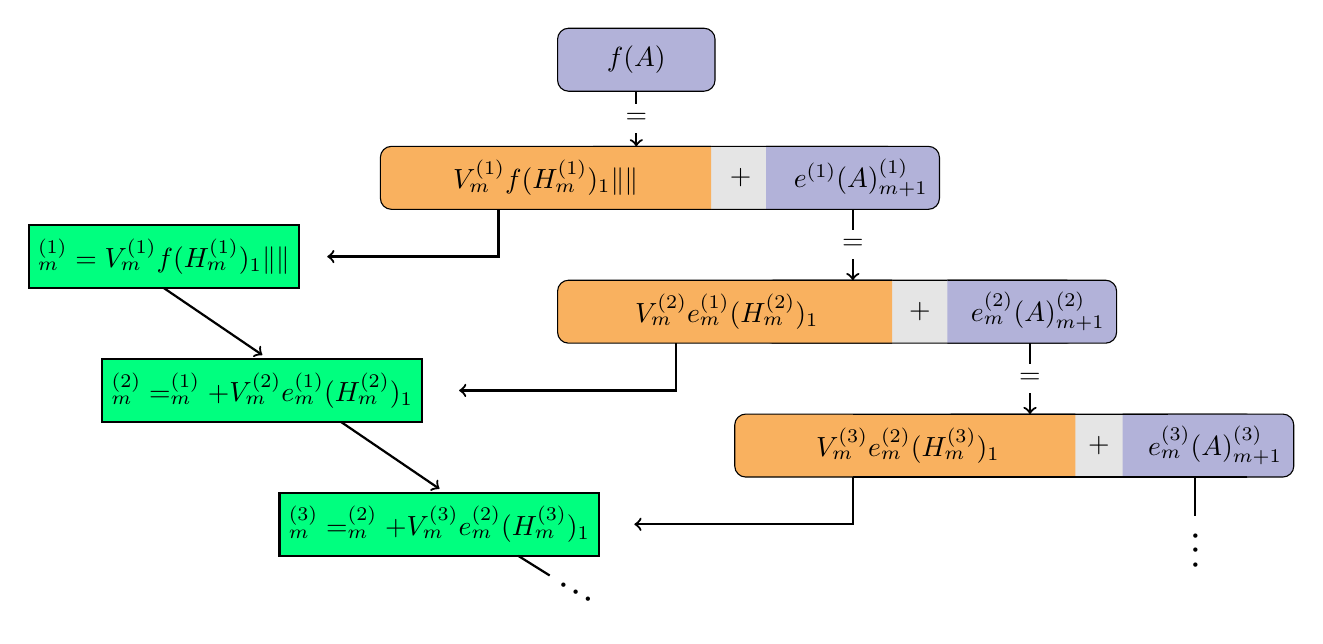
\begin{tikzpicture}
\draw (1.75,0) node[minimum height=0.8cm, minimum width=2cm, draw,fill=NavyBlue!30, rounded corners] {$f(A)\vb$};
\draw[-> , thick] (1.75,-0.4) -- (1.75,-1.1) ;
\draw (1.75,-.75) node[fill=white] {$=$}; 

\draw (3.075,-1.5) node[draw, minimum width = 4cm, minimum height = 0.8cm, fill=gray!20, rounded corners] {$+$};
\draw[fill=BurntOrange!60, rounded corners] (2.7,-1.9) -- (-1.5,-1.9) -- (-1.5,-1.1) -- (2.7,-1.1); 
\draw (0.6,-1.5) node[minimum height=0.8cm, minimum width=3cm] {$V_m^{(1)}f(H_m^{(1)})\ve_1\|\vb\|$};
\draw[fill=NavyBlue!30, rounded corners] (3.4,-1.9) -- (5.6,-1.9) -- (5.6,-1.1) -- (3.4,-1.1);
\draw (4.6,-1.5) node[minimum height=0.8cm, minimum width=2cm] {$e^{(1)}(A)\vv_{m+1}^{(1)}$};

\draw[-> , thick] (0,-1.9) -- (0,-2.5) -- (-2.175,-2.5);
\draw[-> , thick] (4.5,-1.9) -- (4.5,-2.8) ;
\draw (4.5,-2.35) node[fill=white] {$=$};

\draw (5.35,-3.2) node[draw, minimum width = 4cm, minimum height = 0.8cm, fill=gray!20, rounded corners] {$+$};
\draw[fill=BurntOrange!60, rounded corners] (5,-3.6) -- (0.75,-3.6) -- (0.75,-2.8) -- (5,-2.8);
\draw (2.9,-3.2) node[minimum height=0.8cm, minimum width=3cm] {$V_m^{(2)}e_m^{(1)}(H_m^{(2)})\ve_1$};
\draw[fill=NavyBlue!30, rounded corners] (5.7,-3.6) -- (7.85,-3.6) -- (7.85,-2.8) -- (5.7,-2.8);
\draw (6.85,-3.2) node[minimum height=0.8cm, minimum width=2cm] {$e_m^{(2)}(A)\vv_{m+1}^{(2)}$};

\draw[-> , thick] (2.25,-3.6) -- (2.25,-4.2) -- (-.5,-4.2);
\draw[-> , thick] (6.75,-3.6) -- (6.75,-4.5) ;
\draw (6.75,-4.05) node[fill=white] {$=$};

\draw (7.625,-4.9) node[draw, minimum width = 4cm, minimum height = 0.8cm, fill=gray!20, rounded corners] {$+$};
\draw[fill=BurntOrange!60, rounded corners] (7.325,-5.3) -- (3,-5.3) -- (3,-4.5) -- (7.325,-4.5);
\draw (5.2,-4.9) node[minimum height=0.8cm, minimum width=3cm] {$V_m^{(3)}e_m^{(2)}(H_m^{(3)})\ve_1$};
\draw[fill=NavyBlue!30, rounded corners] (7.925,-5.3) -- (10.1,-5.3) -- (10.1,-4.5) -- (7.925,-4.5);
\draw (9.1,-4.9) node[minimum height=0.8cm, minimum width=2cm] {$e_m^{(3)}(A)\vv_{m+1}^{(3)}$};
\draw[-] (4.5,-4.5) -- (8.5,-4.5);
\draw[-] (4.5,-5.3) -- (9.5,-5.3);
\draw[-> , thick] (4.5,-5.3) -- (4.5,-5.9) -- (1.725,-5.9);

\draw[-, thick ] (8.85,-5.3) -- (8.85,-5.8); 
\node at (8.85,-6.2) [rotate=90] {\textbf{\ldots}};

\draw (-4.25,-2.5) node[minimum height=0.8cm, minimum width=0.8cm, draw,fill=SpringGreen, thick] {$\vf_m^{(1)}=V_m^{(1)}f(H_m^{(1)})\ve_1\|\vb\|$};
\draw[->, thick] (-4.25,-2.9) -- (-3.0,-3.75);
\draw (-3,-4.2) node[minimum height=0.8cm, minimum width=0.8cm, draw,fill=SpringGreen, thick] {$\vf_m^{(2)} = \vf_m^{(1)} + V_m^{(2)}e_m^{(1)}(H_m^{(2)})\ve_1$};
\draw[->, thick] (-2,-4.6) -- (-0.75,-5.45);
\draw (-0.75,-5.9) node[minimum height=0.8cm, minimum width=0.8cm, draw,fill=SpringGreen, thick] {$\vf_m^{(3)} = \vf_m^{(2)} + V_m^{(3)}e_m^{(2)}(H_m^{(3)})\ve_1$};
\draw[-, thick] (0.25,-6.3) -- (0.65,-6.55);
\node at (.95,-6.75) [rotate=150] {\textbf{\ldots}};
\end{tikzpicture}}
